\documentclass{report}

\usepackage{a4wide}
\usepackage{amsmath}
\usepackage{amsfonts}
\usepackage[latin1]{inputenc} %input font encoding
\usepackage[T1]{fontenc} % output font encoding
\usepackage{listings}
\usepackage{hyperref}
\usepackage[svgnames]{xcolor}

\usepackage{graphicx}
\graphicspath{{./images/}}

\usepackage{etoolbox} % Add bibliography to toc
\makeatletter
\patchcmd{\thebibliography}{%
  \chapter*{\bibname}\@mkboth{\MakeUppercase\bibname}{\MakeUppercase\bibname}}{%
  \chapter{Bibliography}}{}{}
\makeatother

\hypersetup{
    colorlinks,
    citecolor=DodgerBlue,
    filecolor=black,
    linkcolor=black,
    urlcolor=black
}

\title{Visual Epidemic Simulation}
\author{Matthew Lakin\\\textbf{Supervisor: Hossein Nevisi}}
\date{October 2024 - May 2025}

\begin{document}
\maketitle
\newpage

\tableofcontents


\newpage

\chapter{Abstract}
\begin{center}
    \LARGE{"We've actually invested very little in a system to stop an epidemic. We're not ready for the next epidemic."}
\end{center}
\begin{flushright}
    \large{- Bill Gates, 2015 \cite{gates:2015}}
\end{flushright}
\vspace{0.2cm}In recent years, we have all become too familiar with viruses and epidemics. From Ebola landing in Europe and America in the 2010s after ravaging through Africa, to Covid-19 in the 2020s.\\
New epidemics seem to be springing up at a rate never seen before \cite{morandFigure} and I think there are multiple causes to this.For one, access to medicine has been a huge help in increasing survival rates for all sorts of ailments. However, this has caused complacency in the world of medicine and Antibiotic Resistance, where medicine becomes ineffective to bacterial infections, has become one of the most prevalant issues the human race will face in the coming decades.
Being able to use existing data to predict how epidemics will spread and what


Going back to the 14th Century, the Black Death, or the bubonic plague was one of the worst outbreaks in history. It killed between 75 and 200 million people in a few years time which was 30-50\% of the total population of Europe at the time \cite{dewitte2008selectivity}. 


Smallpox still remains as the only human-affecting virus which has been functionally extinct as a result of human intervention \cite{cdc:smallpox}. This was a result of a combination of mass vaccination, containment and tracking.
In this paper, I wanted to focus on the tracking aspect of containing diseases and how it can be a useful tool to not only teach us about what happened previously, but to predict and forecast what could happen in the future.

\newpage

\chapter{Introduction}
This project intends to create a visual simulation of an epidemic. Using publically available data from the COVID-19 epidemic, the simulation will represent the data in a visual format similar to a dashboard. The simulation will be created using a Dockerised Java environment, with the simulation itself being written in Javascript with node.js.

\newpage

\chapter{Problem Domain}
\section{Minimum Viable Product}
I have identified the minimal requirements for this project to be successful.
\begin{enumerate}
    \item Front end
    \begin{enumerate}
        \item The front end must show a map of the Earth.
        \item The map will render polygon and country data.
        \item The front end must show a timeline of the epidemic.
        \item The individual countries must be clickable.
        \item Clicking a country will show the number of cases and deaths per week.
        \item The user must be able to scrub through the timeline.
        \item The user must be able to select data from a CSV file to be displayed.
    \end{enumerate}
    \item Back end
    \begin{enumerate}
        \item The back end will be using a node.js server.
        \item The epidemic data will be stored in a csv file.
        \item The polygon data will be stored in a GeoJSON file.
        \item The node.js server will be dockerised.
    \end{enumerate}
\end{enumerate}
\newpage
\section{Stretch Goals}
For this project, the following aspirational requirements have been identified:
\begin{enumerate}
    \item Zooming in on the map.
    \item Hotspots on the map.
    \item Predictctive modelling and forecasting.
    \item Analysis of data with other data sources to search for correlations.
\end{enumerate}
\newpage

\chapter{Methodology}
\section{Waterfall}
    For this project I will incorperate a Waterfall model into my project since it will ensure my code and report as a whole is developed in a structured and ordered fashion.\\
    The steps of Waterfall I will be following are:
    \begin{enumerate}
        \item Requirements 
        \begin{itemize}
            \item This section requires producing and refining a set of requirements. I plan on having 2 groups of requirements: Minimum Viable Product requirements and Stretch requirements.
            \item I plan on refining all the requirements in this stage so I can stay on this path plan.
        \end{itemize}
        \item Analysis
        \begin{itemize}
            \item In this section, I will be doing research into the problems which are discovered by my requirement refinement. I will investigate papers and other relevant published sources.
            \item I also want to investigate node packages to represent my data graphically. (This would continue into the design section)
            \item This section will likely take up a large section of my report, and I may return to this section midway through the project.
        \end{itemize}
        \item Design
        \begin{itemize}
            \item I would be designing the layout and colour scheme of my application as it would appear in a browser window. It is worth noting that different size screens would render it differently, so I need to take that into account when planning.
            \item I am not using a database for this project, but I will be using JSON and creating a standard design for objects in JSON will be beneficial.
            \item I need to decide what values I use for graphs and what kind of graphs to use.
        \end{itemize}
        \item Coding
        \begin{itemize}
            \item I will be making a web application with node.js. This will require me to create a valid work environment and get the node runtime working on my local machine. I will likely use Docker for this since it is a very easy to work with tool perfect for this application.
            \item I will mostly be using TypeScript for this project because of type safety and native compatibility with web development. There will also be HTML and CSS for loading the TS canvas and aligning elements.
            \item Node.js also comes with node package manager which will also be useful for loading the custom packages I plan on using in this project.
        \end{itemize}
        \item Testing
        \begin{itemize}
            \item For testing, I will be using a variety of normal, boundary and erroneous tests to check my software for crashes, unexpected results, and vulnerabilities. Using a type-safe language like TypeScript intends to minimise the chances of these happening.
            \item I also plan on having 3rd-party applicants to test my application. They would have a list of things to do in the application so I can analyse the ease of use.
            \item I would also ask them to fill in a questionnaire.
        \end{itemize}
        \item Operations
        \begin{itemize}
            \item I want to deploy my application to a server hosted by the university.
            \item Node.js applications are commonly deployed onto servers and having a production repository would be a good standard for myself. Pushing to a server from a local git repository is a highly transferable skill which is widely used. Test
        \end{itemize}
    \end{enumerate}
\section{Gantt Chart}
    \begin{center}
        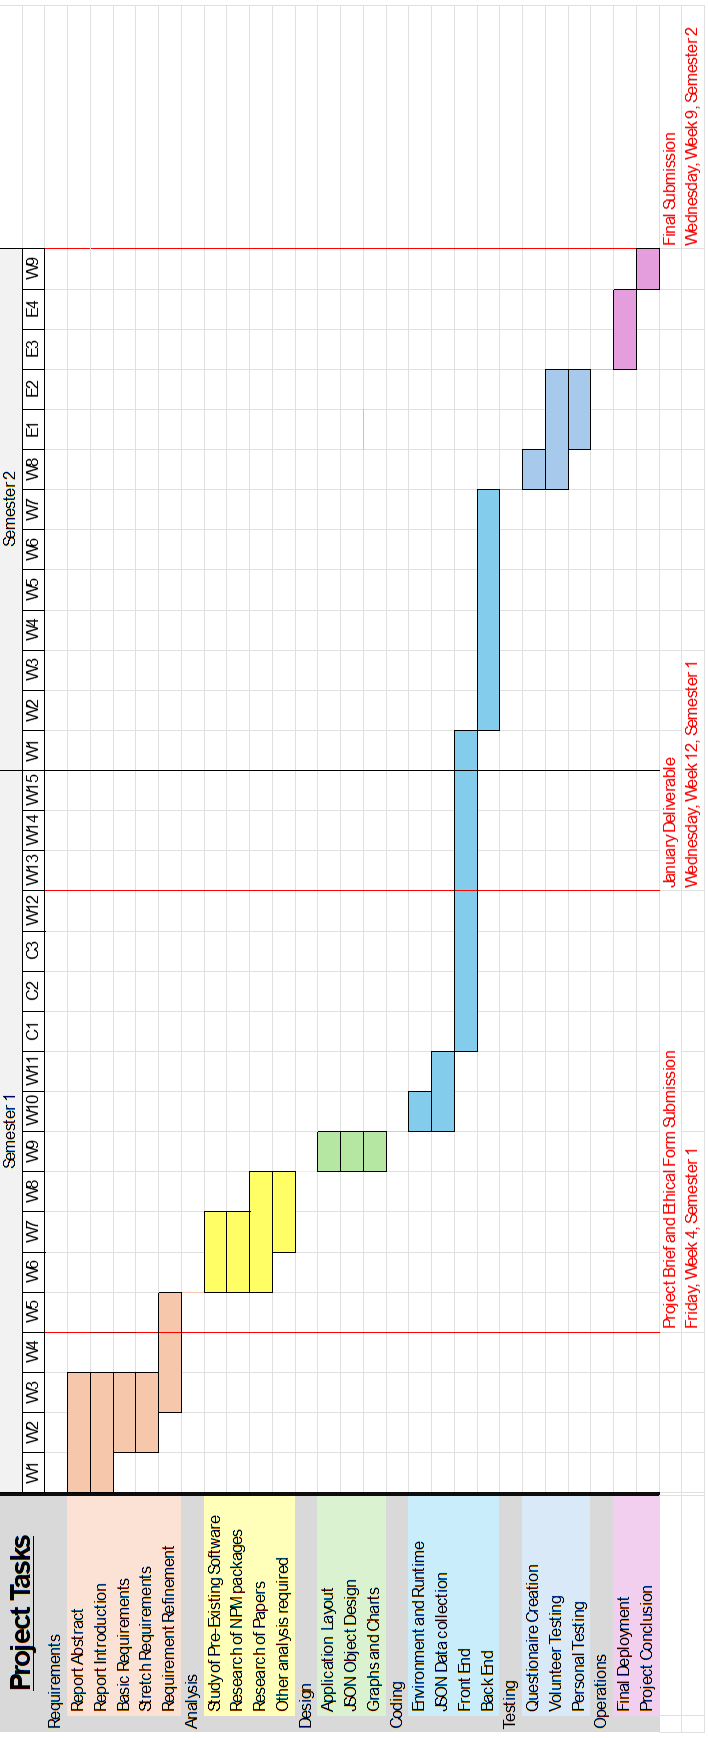
\includegraphics[height=0.95\textheight]{gantt_chart}
    \end{center}

\newpage

\newpage

\chapter{Research}
\section{Existing Solutions}
\subsection{COVID-19 Dashboard}
A common tool for data visualisation is a software called PowerBI, a Microsoft product which allows for the creation of dashboards. 
The dashboard in the figure shows a real-time representation of the COVID-19 pandemic.
\begin{center}
    \begin{figure}[h]
        \centering
        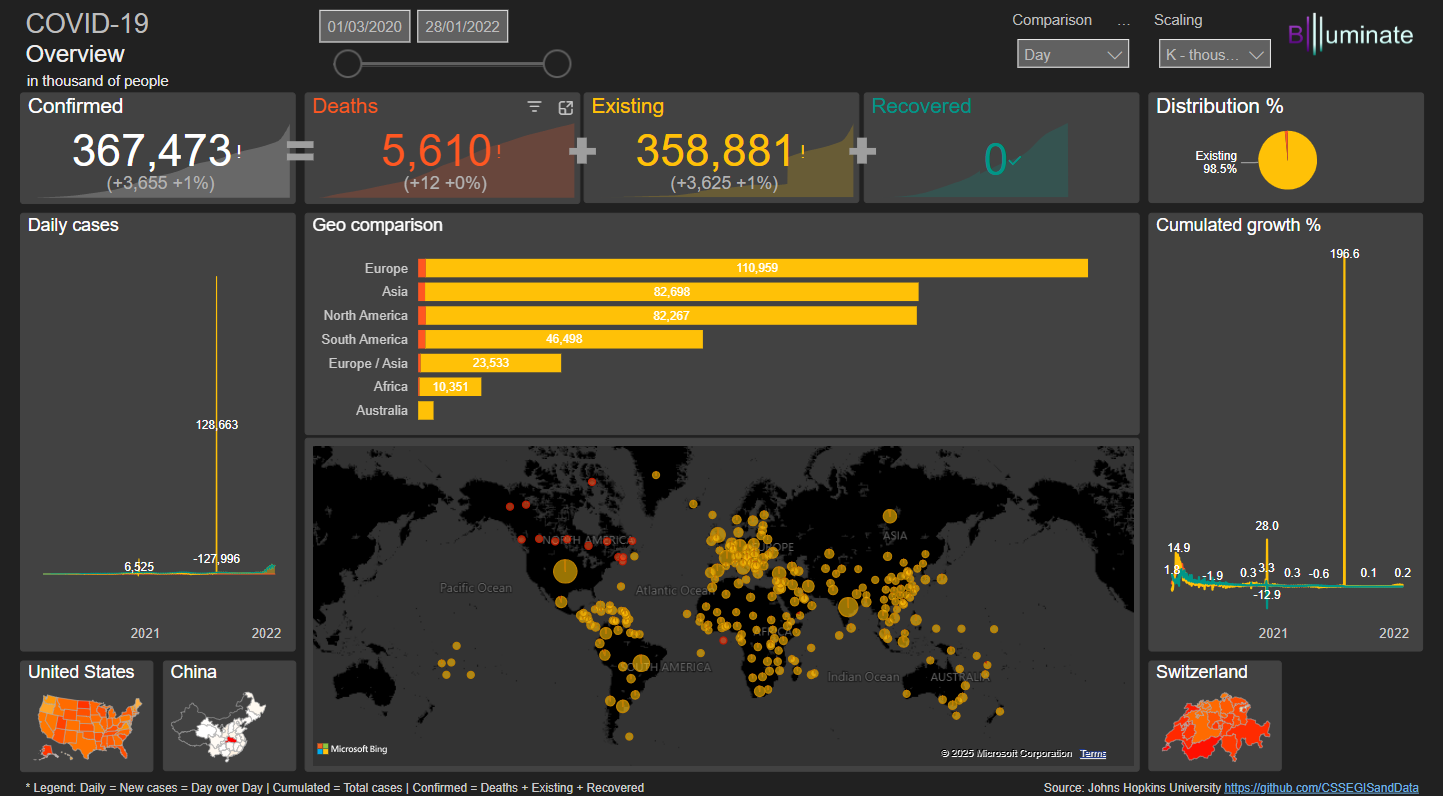
\includegraphics[width=0.95\textwidth]{PowerBI Example.png}
        \caption{COVID-19 Dashboard Example}
        \label{fig:covid19_dashboard}
    \end{figure}
\end{center}

This dashboard has a lot of information on it even at first glance. The map uses bubbles to denote hotspots of activity for the virus. The bubbles are sized by the number of cases in that country. The bubbles can also be clicked for more detailed information on that country. \\
The user is also able to alter the time frame of the data, and the data is updated in real time.\\
\newpage
\subsection{Plague Inc.}
Plague Inc. is a game published in 2012 by Ndemic Creations. It gives the user the ability to create and spread a virus across the world. The game was initially released on mobile devices and has since been released on PC and console.\\
Mobiles games require accessible and easy to use interfaces, which is why Plague Inc. is a good example of a visual epidemic simulation. The game is simple to use and has a lot of information on the screen at once.
\begin{center}
    \begin{figure}[h]
        \centering
        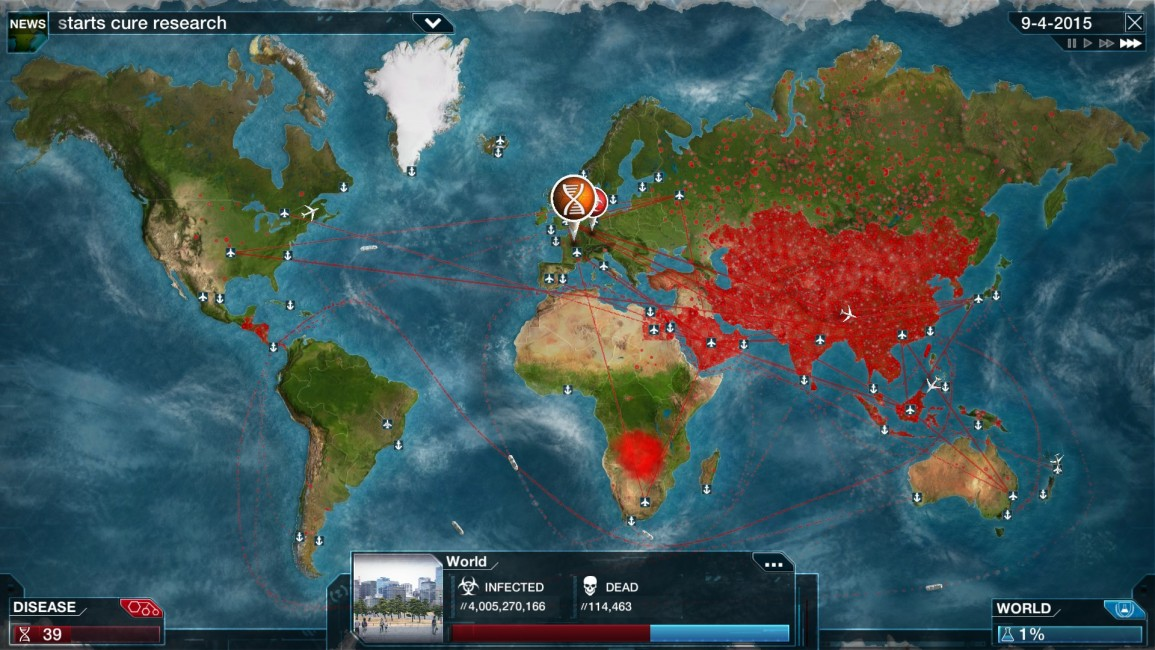
\includegraphics[width=0.95\textwidth]{Plague Inc Example.jpeg}
        \caption{Plague Inc. Dashboard Example}
        \label{fig:plagueinc_dashboard}
    \end{figure}
\end{center}
Despite many systems being dramatised for the sake of gameplay, the game offers many features which could be useful for a real-world epidemic simulation. \\
The game uses a world map which gradually changes colour as the virus spreads, this is from many red dots appearing on the map. The user also has access to individual breakdowns of each country and can see the number of cases and deaths in each country.\\ 
The game also has a transmission system which changes from coutnry to country. 

\section{Compartmental Models}
Compartmental models are a type of mathematical model used to represent the different populations in a system. The most common compartmental system in epidemiology is the SIR model.\\
The SIR model is a simple model which divides the population into three compartments: Susceptible, Infected and Recovered. The model is represented by the following differential equations:
\begin{align}
\frac{dS}{dt} &= -\alpha SI \\
\frac{dI}{dt} &= \alpha SI - \beta I \\
\frac{dR}{dt} &= \beta I
\end{align}
\cite{beckley2013modeling}

\chapter{Technical Solution}

\newpage

\chapter{Results and Analysis}
\newpage

\chapter{Conclusion}
\newpage

\bibliographystyle{plain} % We choose the "plain" reference style
\bibliography{refs} % Entries are in the refs.bib file


\newpage

\chapter{Appendix}

\newpage




\end{document}